
%(BEGIN_QUESTION)
% Copyright 2006, Tony R. Kuphaldt, released under the Creative Commons Attribution License (v 1.0)
% This means you may do almost anything with this work of mine, so long as you give me proper credit

A simple way to make a {\it micromanometer} (an extremely sensitive manometer) is to connect two large-diameter vertical tubes by a small-diameter, transparent tube with an air bubble in it.  The air bubble becomes the marker for reading pressure along a scale:

$$\includegraphics[width=15.5cm]{i00169x01.eps}$$

If both of the large vertical tubes are 2.5 inches in diameter, and the transparent, horizontal tube is 0.25 inches in diameter, how much differential pressure will be indicated by 1 inch of horizontal bubble displacement?  Assume the use of water for the manometer liquid.

\underbar{file i00169}
%(END_QUESTION)





%(BEGIN_ANSWER)

1 inch of bubble motion represents 0.02 inches of water column pressure (differential), or 2/100 "W.C., applied across this micromanometer.

\vskip 10pt

To solve for this pressure, first determine the amount of liquid volume that would have to be displaced to move the bubble 1 inch.  Since the bubble resides in a tube 0.25 inches in diameter, the volume for 1 inch of bubble motion is:

\vskip 10pt

(1 inch)[$\pi$(0.25 inch / 2)$^{2}$] = 0.04909 in$^{3}$

\vskip 10pt

This is a very small amount of liquid volume!  The water levels in the larger (2.5 inch diameter) tubes will not have to change much to accommodate this tiny amount of displacement.  Dividing the displaced fluid volume by the area of the vertical tubes will tell us how far the water levels must change in each of the vertical tubes:

\vskip 10pt

(0.04909 in$^{3}$) / [$\pi$(2.5 inch / 2)$^{2}$] = 0.01 inch

\vskip 10pt

So, a vertical liquid column height change of only 0.01 inch will cause a horizontal bubble displacement of 1 inch.  Since there will be 0.01 inch of movement in {\it each} vertical tube, the combined total vertical displacement is twice this figure, or 0.02 inches of water column.

A much simpler way to solve this problem is to recognize that the vertical tube areas are 100 times as great as the horizontal tube (2.5 inches is ten times as large as 0.25 inches, and area is proportional to diameter {\it squared}), so 1 inch of horizontal fluid displacement is proportional to 1/100 inch of vertical fluid displacement.  Once again, since {\it each} vertical tube experiences 0.01 inch of vertical water level displacement, the total water column shift is 0.02 inches.


%(END_ANSWER)





%(BEGIN_NOTES)


%INDEX% Measurement, pressure: micro-manometer

%(END_NOTES)


